% !TEX encoding = UTF-8 Unicode

\documentclass{standalone}

% packages
\usepackage{float}
\usepackage{tabu}
\usepackage{booktabs}
\usepackage{graphicx}
\usepackage{caption}
\usepackage[export]{adjustbox}
\usepackage[utf8]{inputenc}
%\usepackage[active,pdftex,tightpage]{preview}
\usepackage{newtxtext,newtxmath}
\usepackage[percent]{overpic}

\begin{document}

%\sf
\tiny
\centering 

% Steady state SIMWE simulations

\begin{tabular}{m{0.5\textwidth} m{0.5\textwidth}}
%
\multicolumn{1}{c}{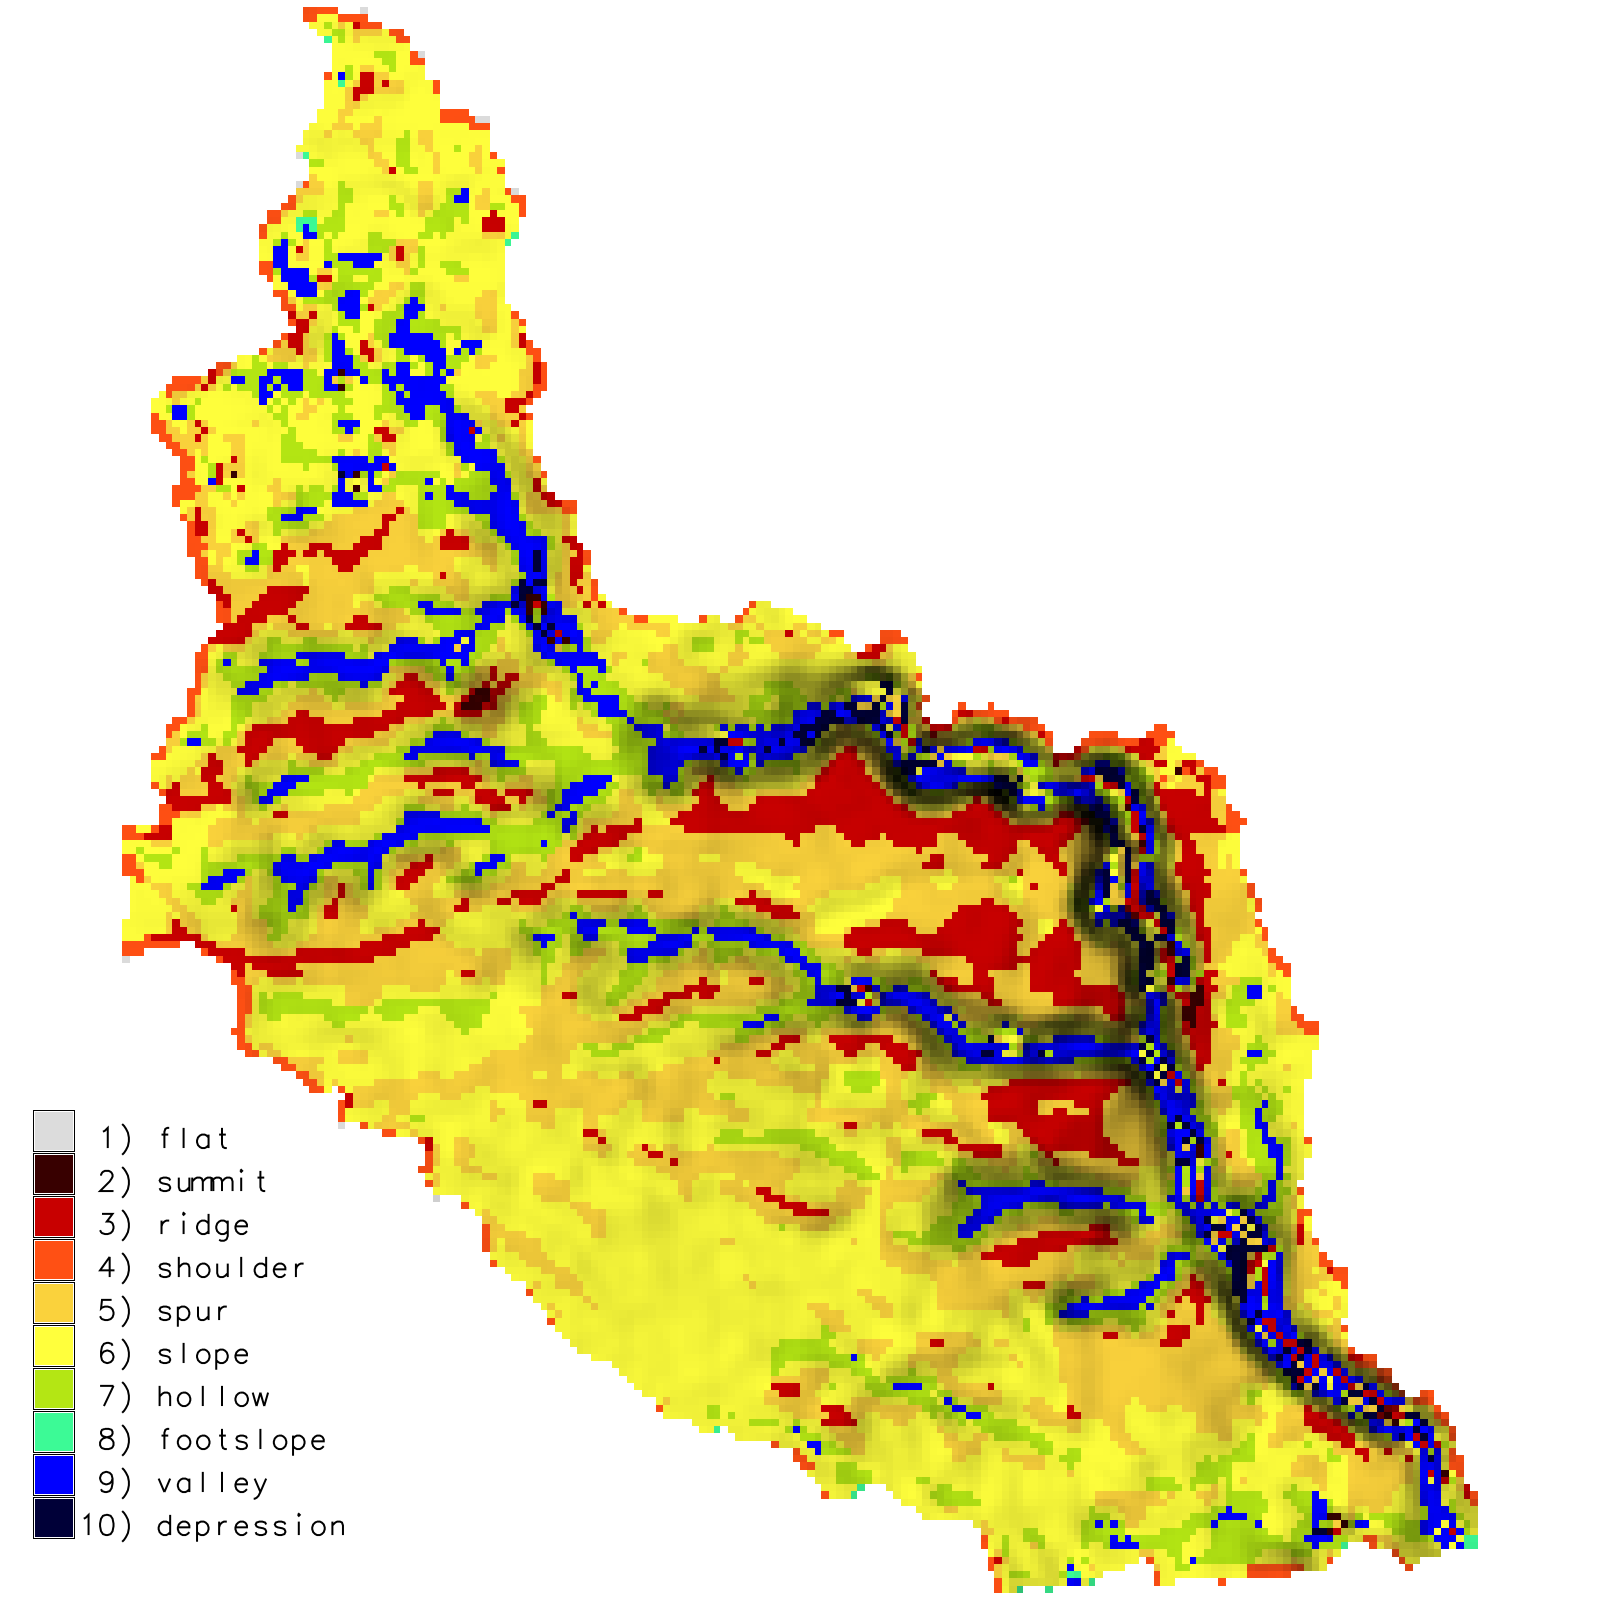
\includegraphics[height=50mm]{../../images/ss_erdep_detail/landforms.png}}
& \multicolumn{1}{c}{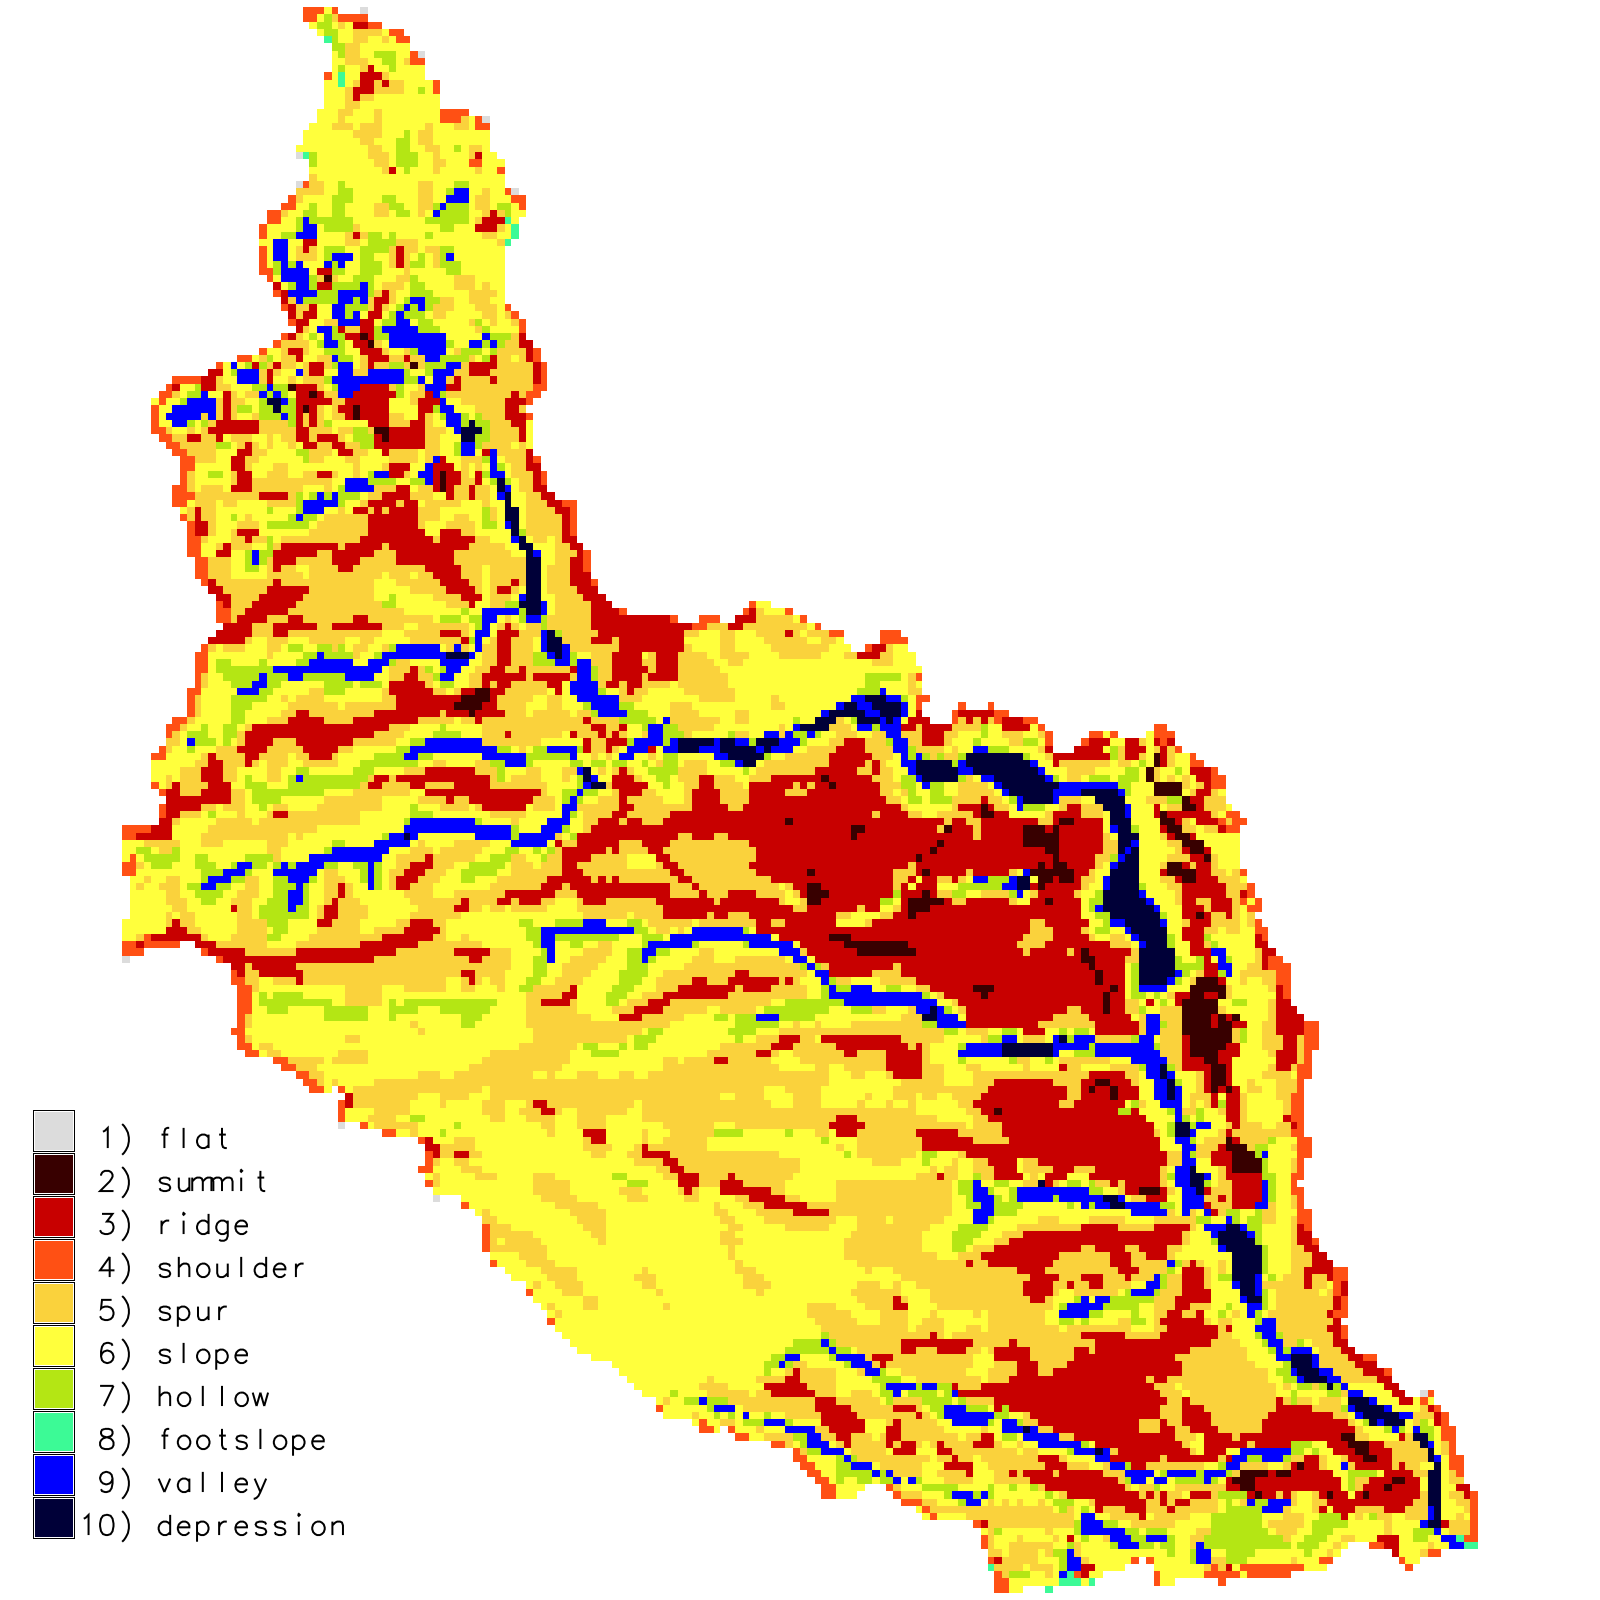
\includegraphics[height=50mm]{../../images/ss_flux_detail/landforms.png}}\\
\\
\\
\multicolumn{1}{c}{a. Erosion-deposition simulation landforms}
& \multicolumn{1}{c}{c. Detachment limited landforms}\\
\\
\\
\multicolumn{1}{c}{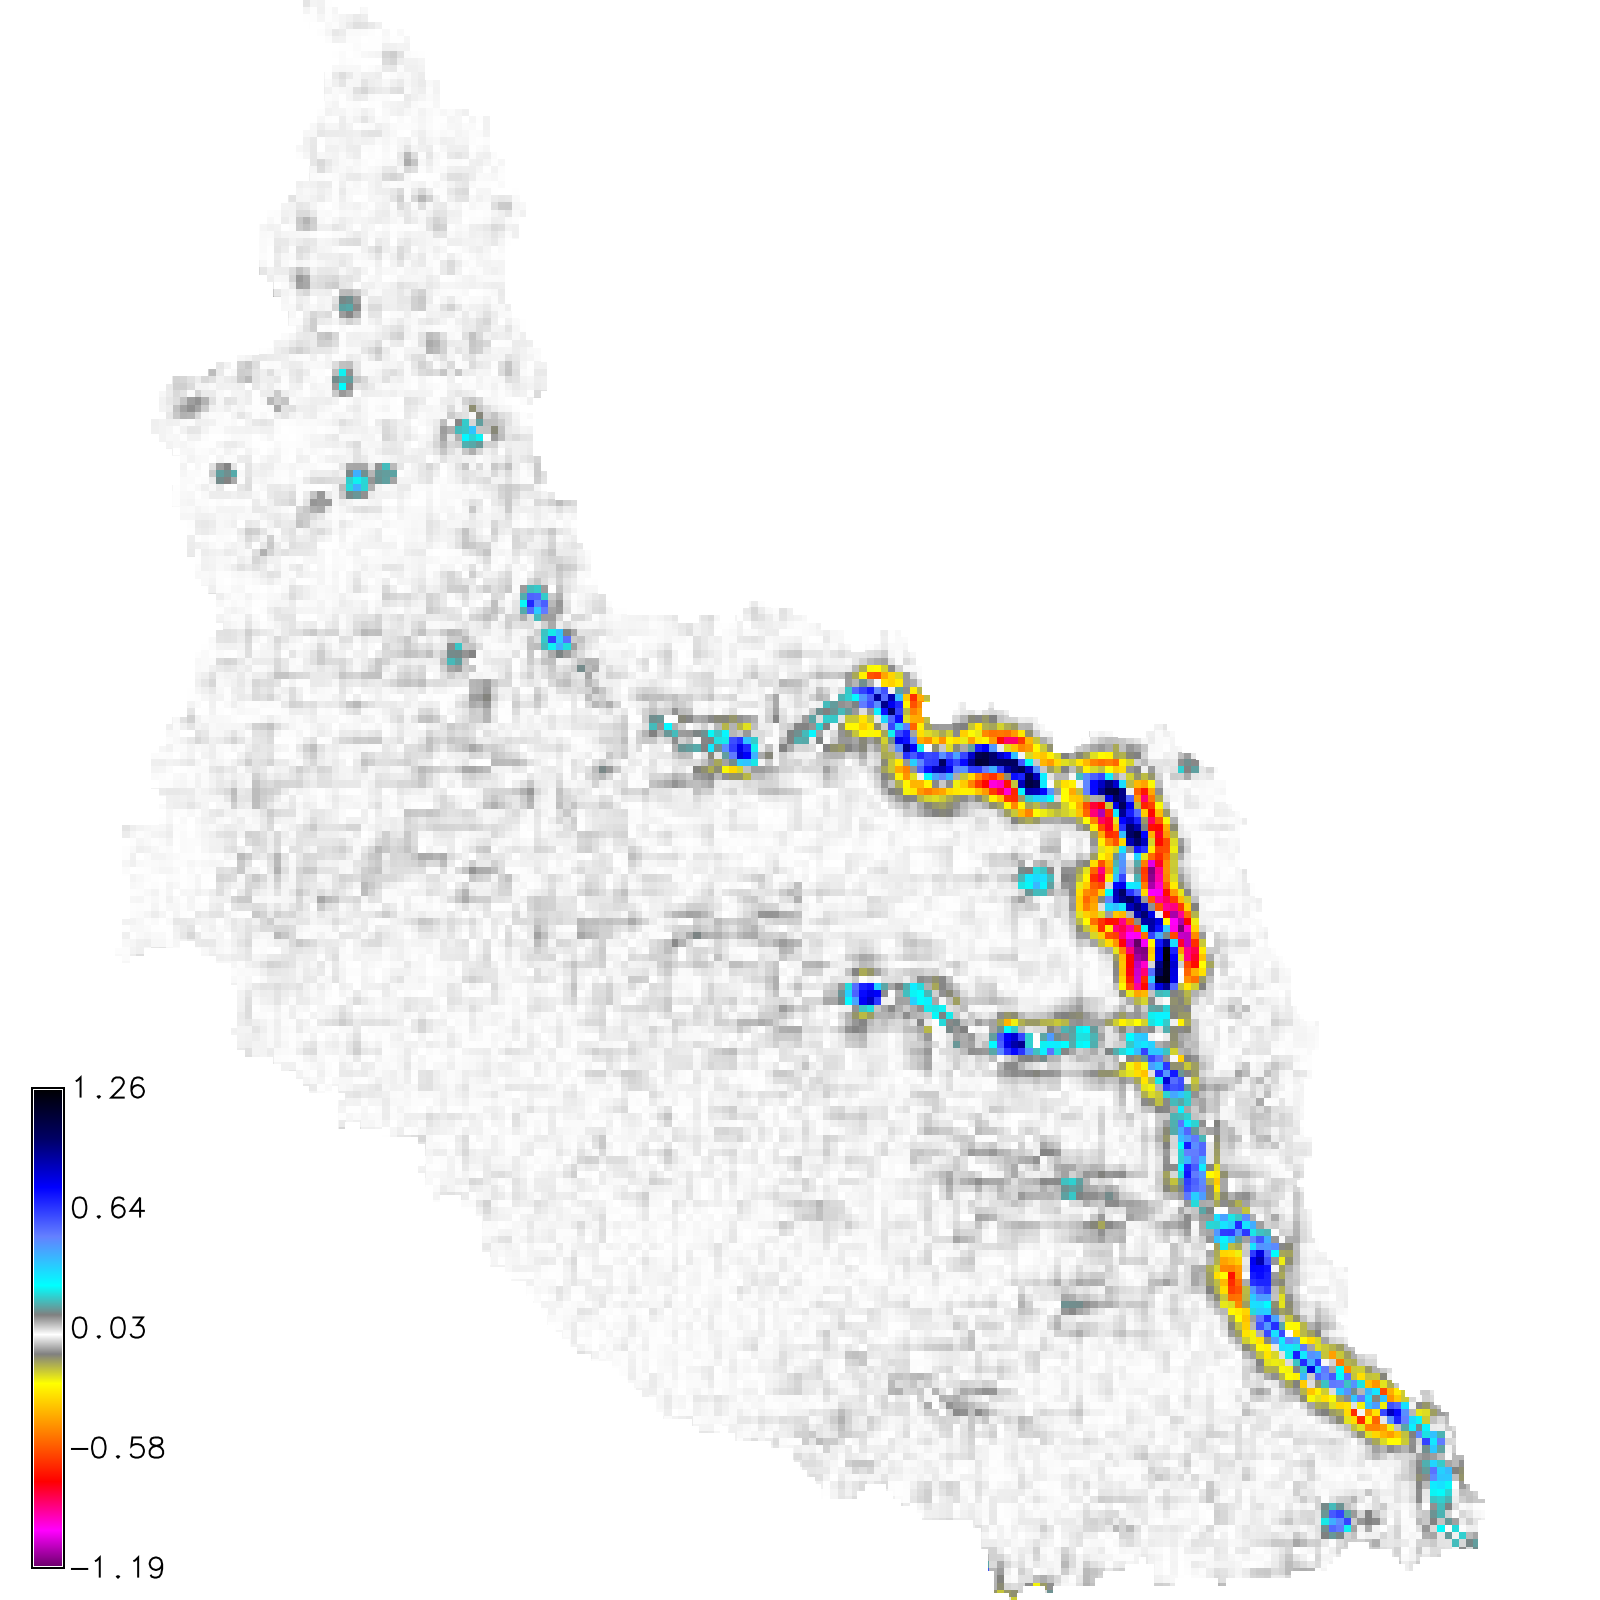
\includegraphics[height=50mm]{../../images/ss_erdep_detail/net_difference.png}}
%& \multicolumn{1}{c}{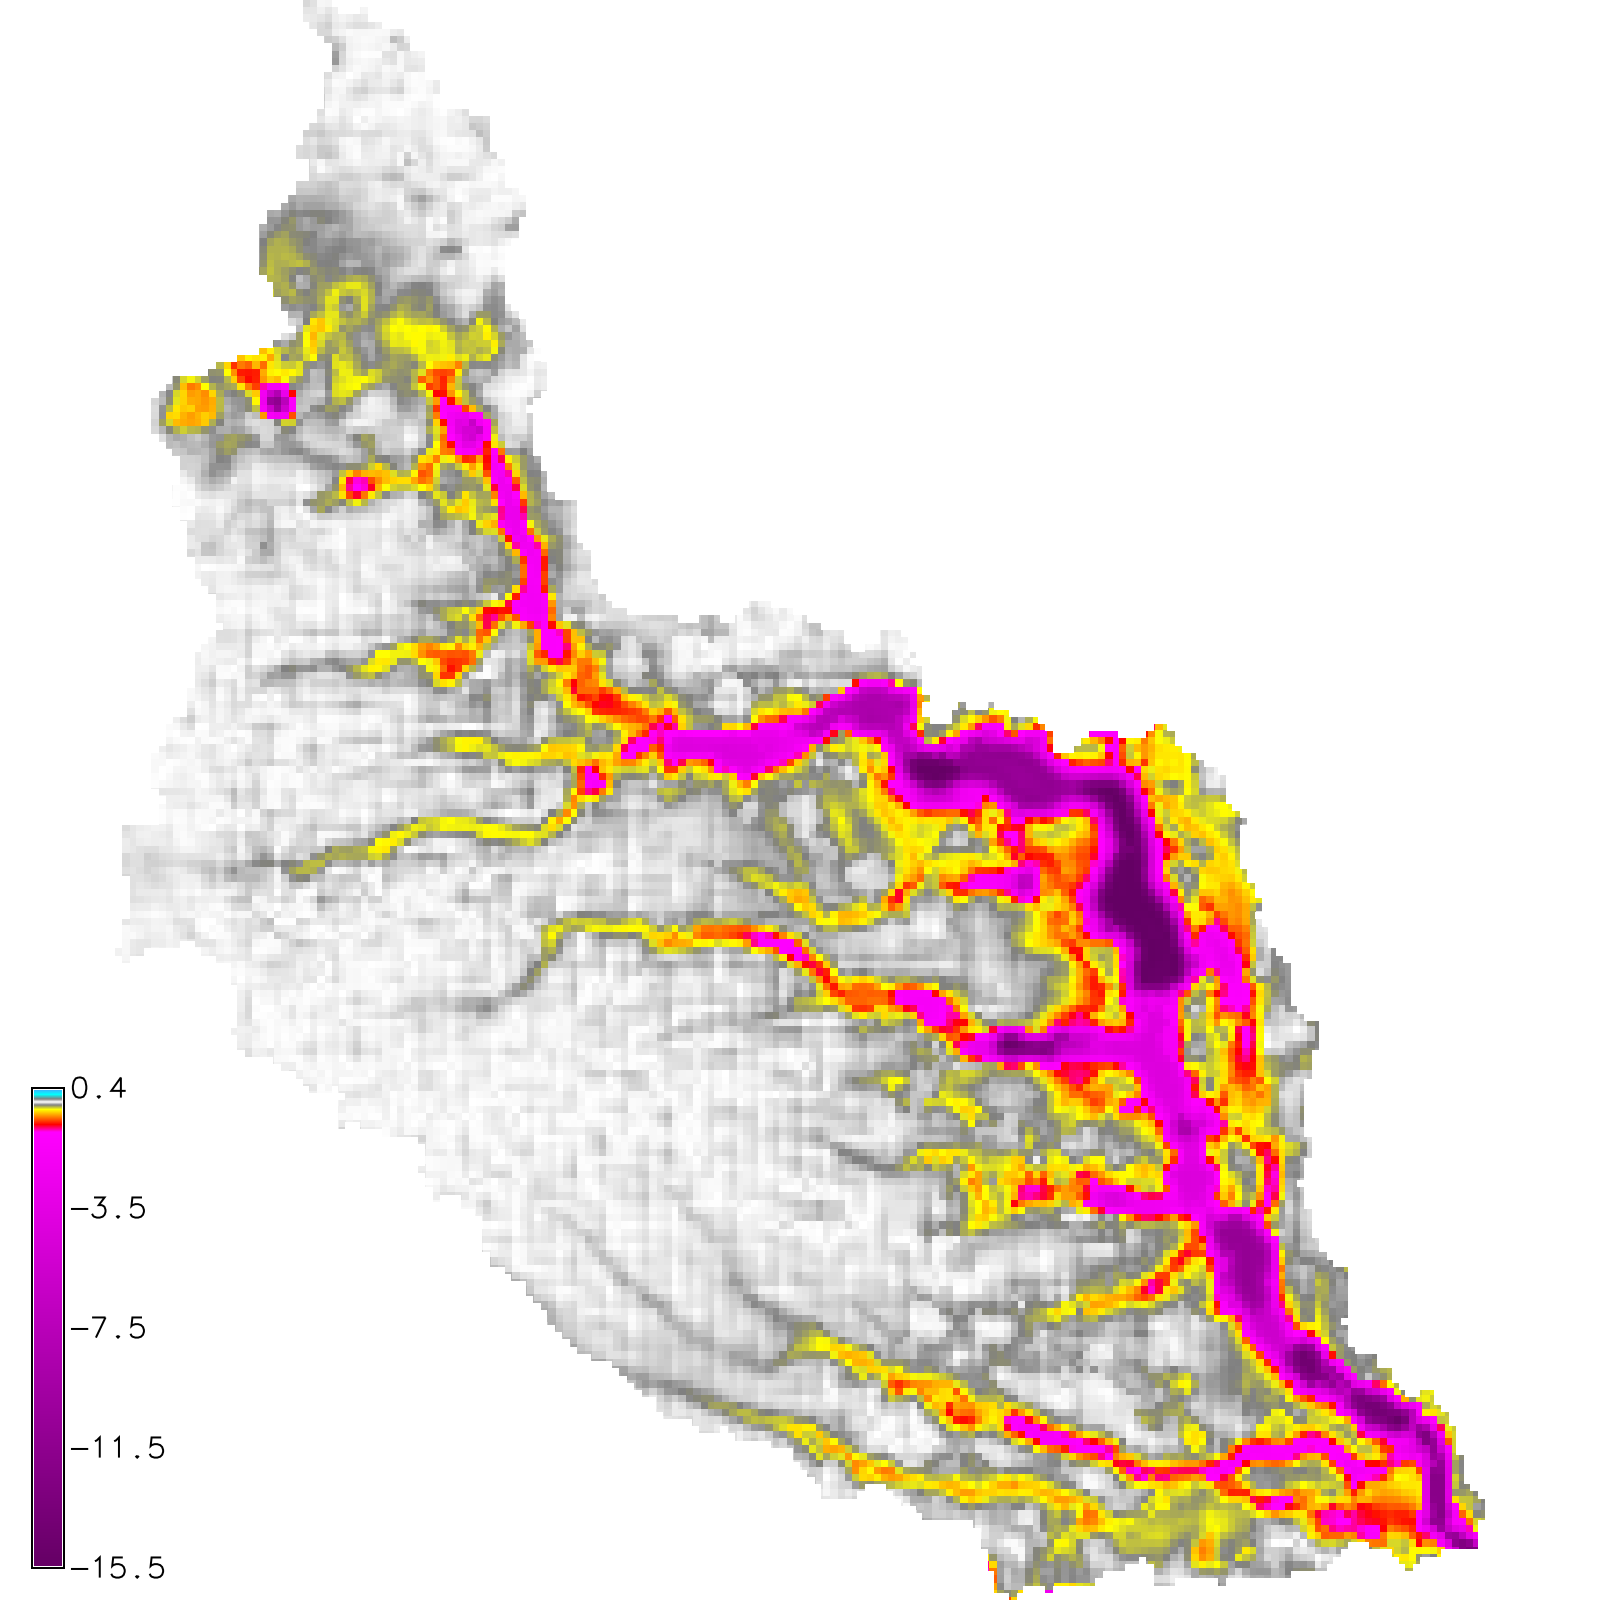
\includegraphics[height=50mm]{../../images/ss_flux_detail/net_difference.png}}\\
& \multicolumn{1}{c}{\begin{overpic}[height=50mm]{../../images/ss_flux_detail/net_difference.png}
\put(-28,-15){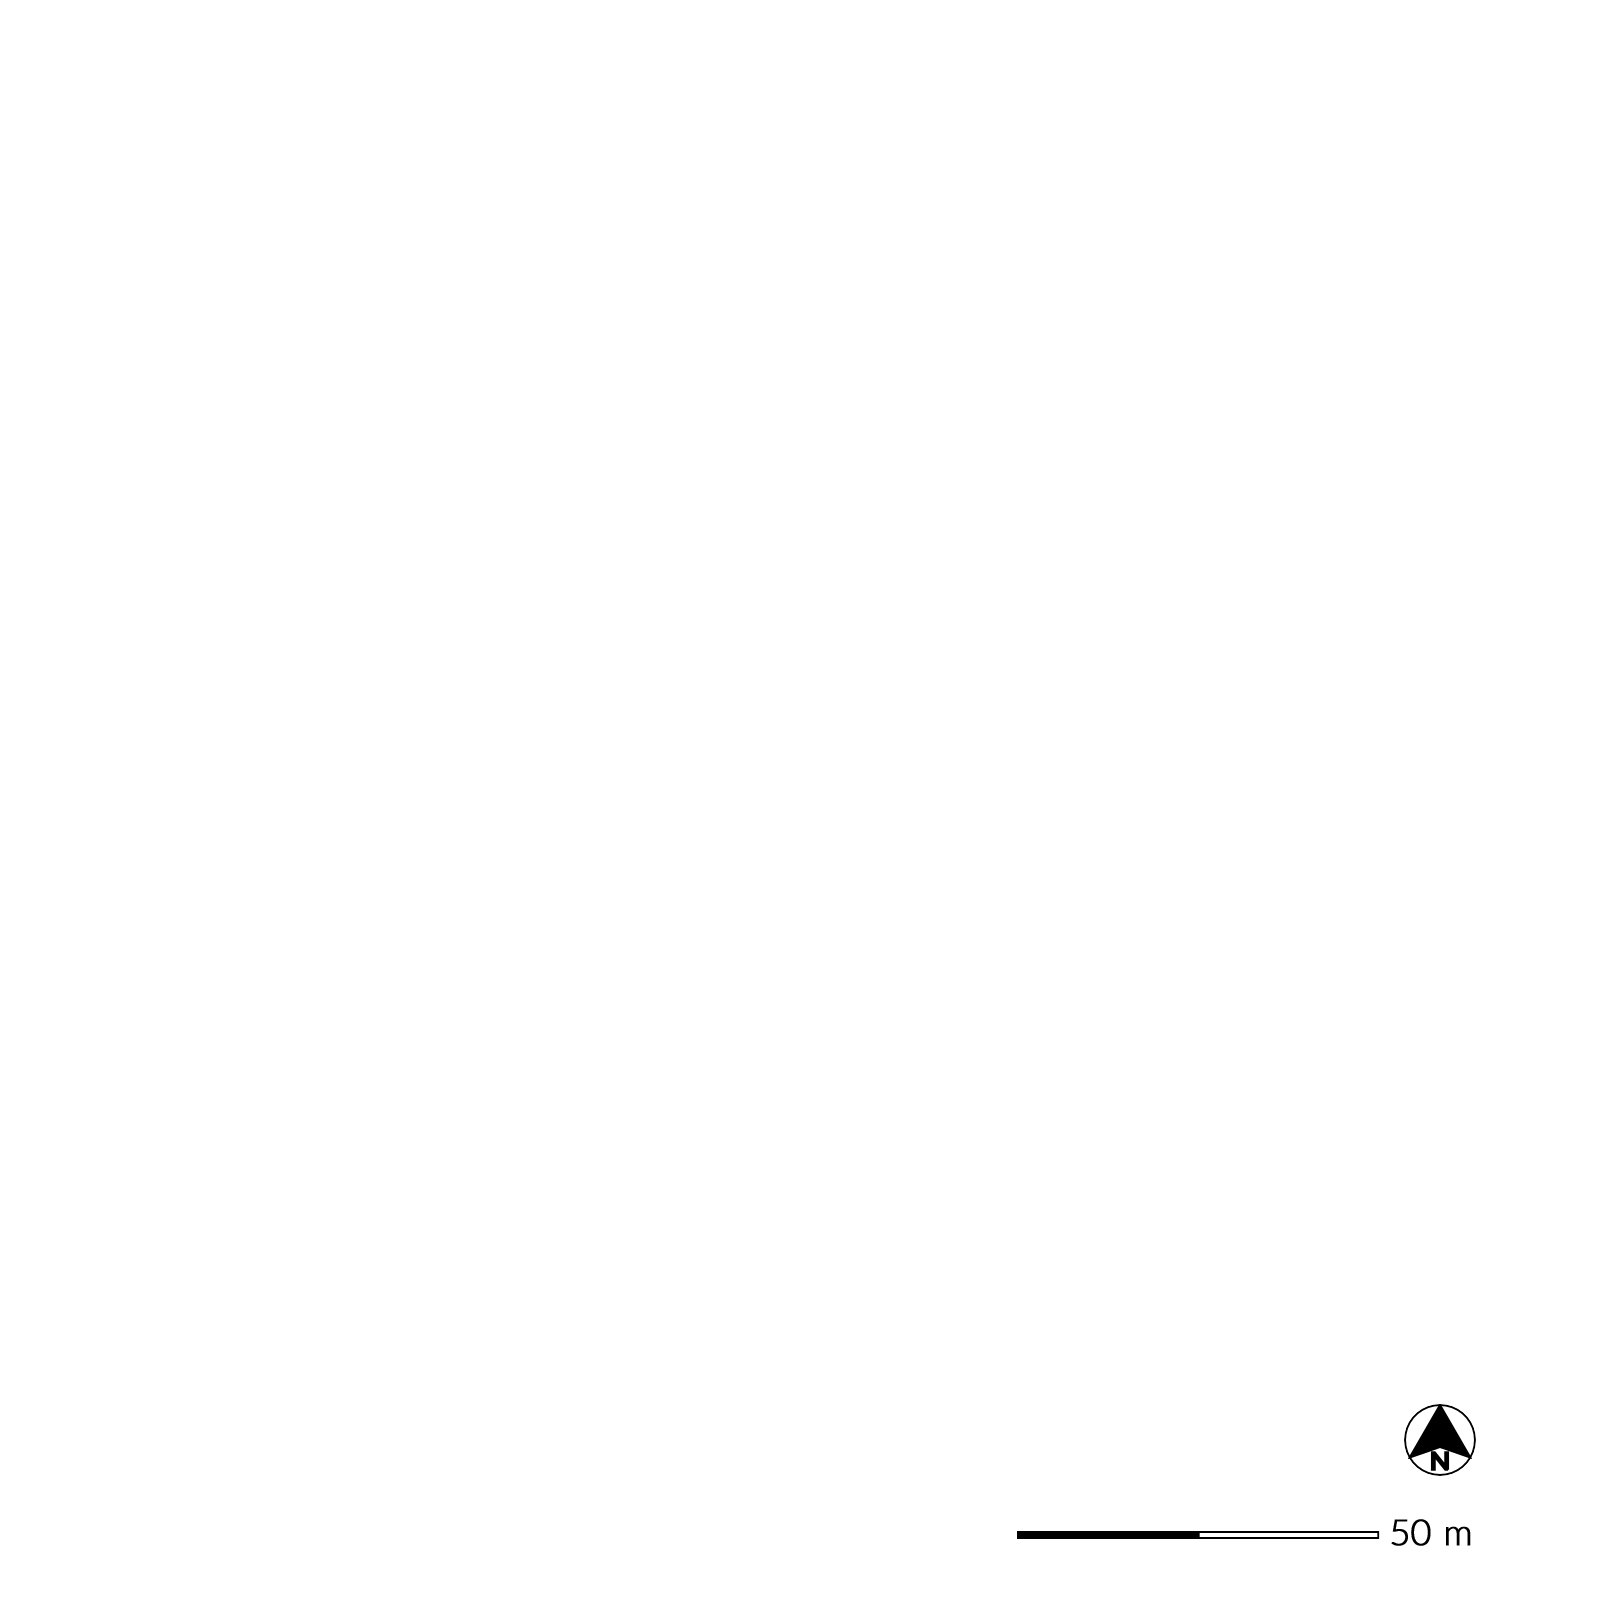
\includegraphics[height=70mm]{../../images/sample_data/map_elements_detail.png}}  
\end{overpic}}\\
\\
\\
\\
\multicolumn{1}{c}{b. Erosion-deposition simulation net difference [m]} 
& \multicolumn{1}{c}{d. Detachment limited simulation net difference [m]}\\
\end{tabular}

\end{document}

